% 2026年北京高考数学第18题：直三棱柱与折线
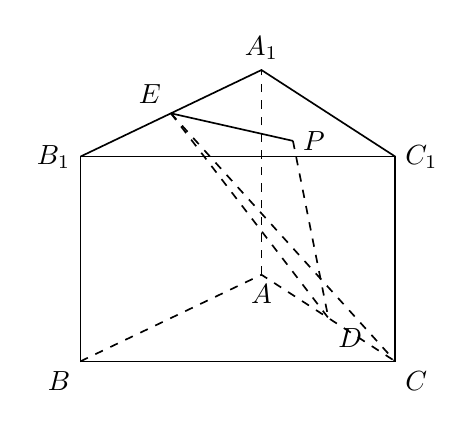
\begin{tikzpicture}[>=stealth,line width=0.6pt,font=\normalsize]
  \coordinate (B) at (0,0);
  \coordinate (C) at (4.0,0);
  \coordinate (A) at (2.3,1.1);
  \coordinate (B1) at (0,2.6);
  \coordinate (C1) at (4.0,2.6);
  \coordinate (A1) at (2.3,3.7);

  \coordinate (E) at (1.15,3.15);
  \coordinate (D) at (3.15,0.55);
  \coordinate (P) at (2.7,2.8);

  % 实线可见边
  \draw (B) -- (C) -- (C1) -- (B1) -- cycle;
  \draw (B1) -- (A1) -- (C1);
  \draw (E) -- (P);

  % 虚线不可见边与内部线
  \draw[dashed] (B) -- (A) -- (C);
  \draw[dashed] (A) -- (A1);
  \draw[dashed] (E) -- (D);
  \draw[dashed] (P) -- (D);
  \draw[dashed] (E) -- (C);

  % 顶点标注
  \node[left] at (B1) {$B_1$};
  \node[right] at (C1) {$C_1$};
  \node[above] at (A1) {$A_1$};
  \node[below left] at (B) {$B$};
  \node[below right] at (C) {$C$};
  \node[below] at (A) {$A$};
  \node[above left] at (E) {$E$};
  \node[below right] at (D) {$D$};
  \node[right] at (P) {$P$};
\end{tikzpicture}
